The two models have been built in COMSOL Multiphysics. \\
The structures have been divided into five different domains (\autoref{fig:microphone_structure}):

\begin{itemize}
    \item \textbf{Diaphragm}: The membrane on which the pressure is applied
    \item \textbf{Backplate}: The bottom plate
    \item \textbf{Lateral borders}: The two insulating lateral spacers that separate the backplate from the diaphragm (every border is a separate domain)
    \item \textbf{Air gap}: The air region between the diaphragm and the backplate
\end{itemize}

\begin{figure}[h!]
    \centering
    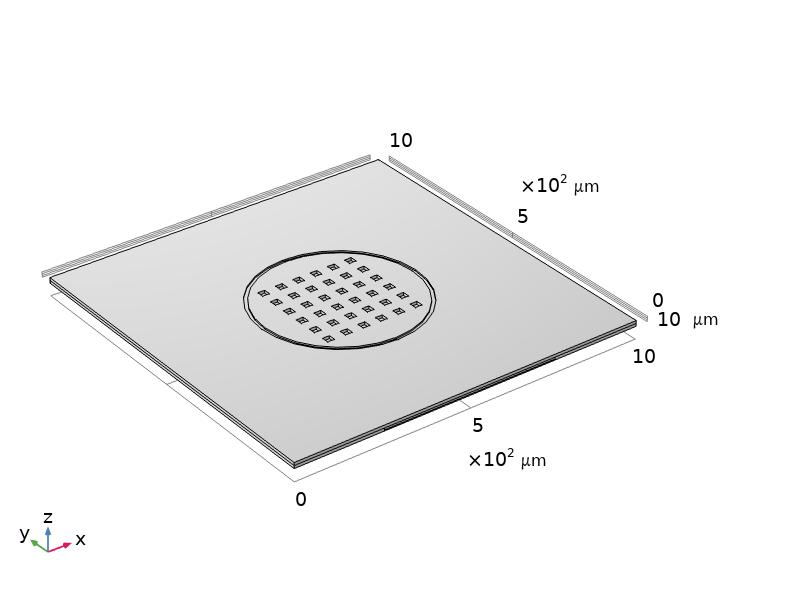
\includegraphics[width=0.95\linewidth]{img/microphone_structure.jpg}
    \caption{Microphone with perforated diaphragm model in COMSOL 6.4}
    \label{fig:microphone_structure}
\end{figure}

\newpage
\noindent
After defining the model structure and domains, the materials have been assigned:

\begin{itemize}
    \item The diaphragm and the bottom plate are made of aluminum
    \item The lateral borders are made of silicon dioxide ($SiO_2$)
    \item The gap between the diaphragm and the bottom plate is filled with air
\end{itemize}

\noindent
The final step in completing the model definition is to define the air gap as a moving mesh. \\
The top and lateral dimensions of the structure are shown in \autoref{fig:top_dimensions} and \autoref{fig:lateral_dimensions}, respectively.

\begin{figure}[h!]
    \centering
    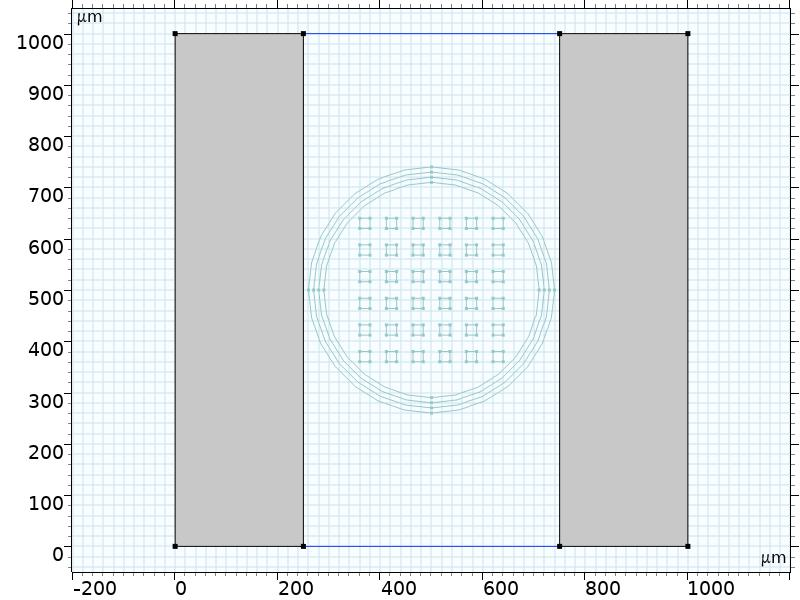
\includegraphics[width=0.95\linewidth]{img/top_dimensions.jpg}
    \caption{Top view of the MEMS microphone structure showing the main geometric dimensions in COMSOL 6.4.}
    \label{fig:top_dimensions}
\end{figure}

\begin{figure}[h!]
    \centering
    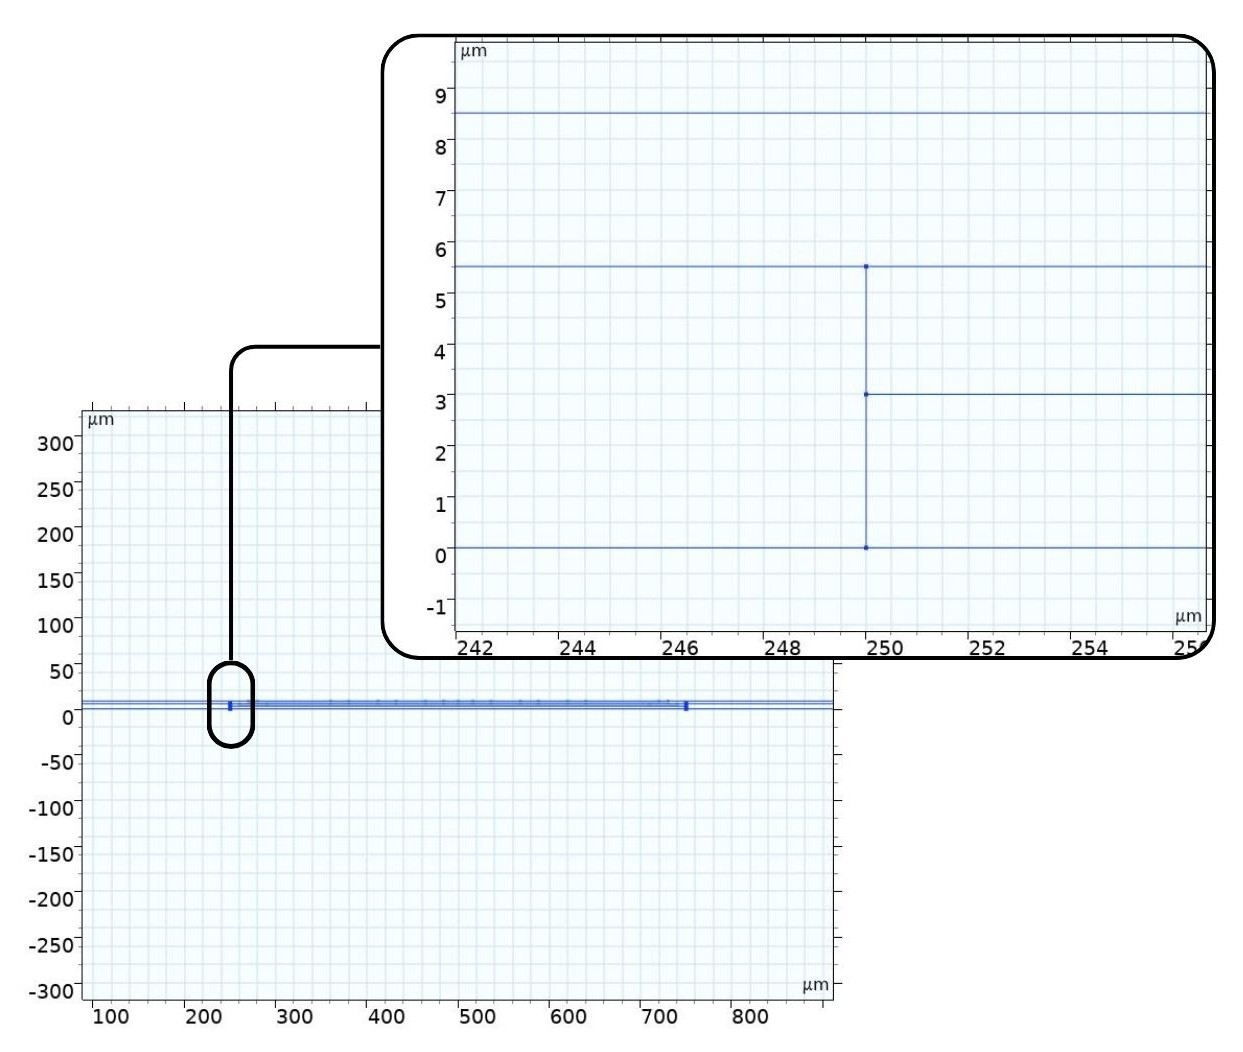
\includegraphics[width=0.95\linewidth]{img/lateral_dimensions.jpg}
    \caption{Lateral view of the MEMS microphone structure highlighting the vertical dimensions in COMSOL 6.4.}
    \label{fig:lateral_dimensions}
\end{figure}
